\chapter{The Dashboard Solution}\label{ch:solution}

\section*{}

In this chapter, we will describe the Dashboard solution, its implementation and methodology under its development.

Since Synopsys had already setup the CI server in Jenkins, it was chosen to develop the Plugin for it. We also take the avantage of Jenkins being very customizable, with hundreds of extension points and plugins available to support our needs~\cite{kn:Jenkins}~\cite{jnks:extensionpoints}.

Nonetheless, it is not a simple task to develop a plugin due to lack of documentation. In order to find out how plugins work, it was crucial to look into other plugins source code.

Our plugin, named \textbf{Filtered Dashboard View} plugin~\cite{jksn:myplugin}, will be referenced from here on simply as \textbf{Dashboard}.

\section{Use Cases}\label{sc:usecases}

Taking into consideration the R\&D project organization of Jenkins, described in section \ref{sc:projOrg}, it was discussed with the collaborating IPK team that the best option was to develop the Dashboard as a View plugin, implementing the class ViewGroup, in order to aggregate different views inside it.

In the Use Case diagram in the figure ~\ref{fig:usecases} are pictured the actions a user can perform to display our Dashboard in the Jenkins environment. 

\newcommand{\code}{\texttt}



\begin{figure}
  \centering
      \makebox[\textwidth][c]{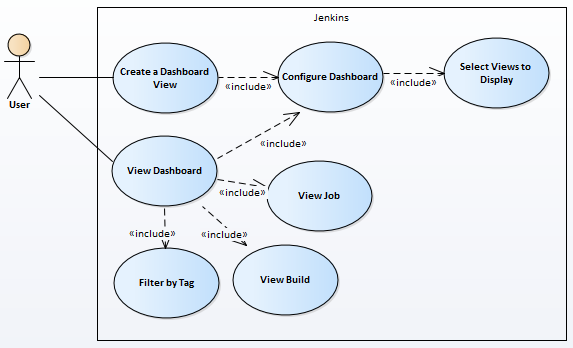
\includegraphics[width=1\textwidth]{usecases}}
      \caption{Dashboard plugin Use Case diagram}
      \label{fig:usecases}
\end{figure}  

The plugin is designed to be as simple as creating a new View inside the tool, selecting which other Views are requested to display, as shown in the figure \ref{fig:createView}. Afterwards, the user can freely change its configuration, namely add, remove or change which views will be displayed, demonstrated in the figure~\ref{fig:customize}.

It is important to note that all kinds of Views should be allowed to display inside the Dashboard, with the exception of itself and other instances of the same View Class, so no loops are originated from this process. 


    \begin{figure}[H]
        \begin{minipage}[b]{0.45\linewidth}
            \centering
            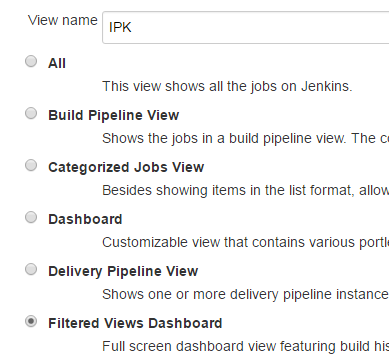
\includegraphics[width=\textwidth]{newview}
            \caption{View creation menu}
            \label{fig:createView}
        \end{minipage}
        \hspace{0.5cm}
        \begin{minipage}[b]{0.45\linewidth}
            \centering
            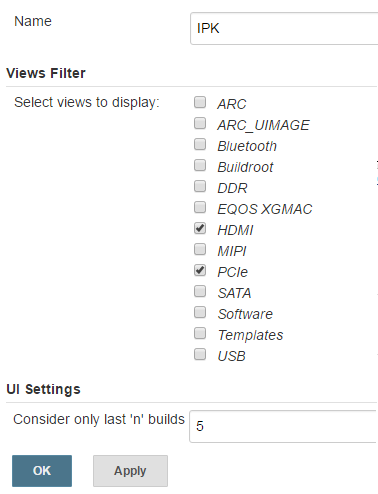
\includegraphics[width=\textwidth]{customiseview}
            \caption{Dashboard customization menu}
            \label{fig:customize}
        \end{minipage}
    \end{figure}

\section{Jenkins Plugin - Filtered Dashboard View}\label{sc:dashboard}

In this section it will be described the thought process of designing our plugin, including the research of similar and auxiliary plugins in \ref{sc:aux}, our implementation design in section~\ref{sc:implementationDesign}, and finally the display of the User Interface of the final product in section~\ref{sc:ui}.


\subsection{Auxiliary Plugins}\label{sc:aux}

Since Jenkins~\citet{kn:Jenkins} supports plugins, with an abundance of extension points which allow it to be extended to meet specific needs of individual projects, it was appropriate to investigate what similar plugins already exist that can be extended or modified as base to our own solution.

In this section, it will be described 2 plugins used to help achieve our final application.

\subsubsection{Mission Control Plugin}\label{mission_plugin}

Accounting that we want to create a Dashboard, we came across the Mission Control Plugin~\cite{jkns:missionC}, that has practically all the base to work with, a full dashboard view that features:

\begin{itemize}
\item Job status display;
\item Build history and build queue;
\item Extends a View Object~\cite{jnks:ViewObj}, which can be added to the main dashboard.
\end{itemize}

Despite being a starting point, the information displayed in the figure \ref{fig:missionControl}, needed to be trimmed and adapted to our requirements. 

Nevertheless, after making a profound source code analysis of this plugin, we had a good understanding on how we could interact with the Jenkins API in various ways, such as retrieving information of all necessary items in our Jenkins instance, exportation of this information and its interaction with the front-end.

  \begin{figure}[H]
  \centering
      \makebox[\textwidth][c]{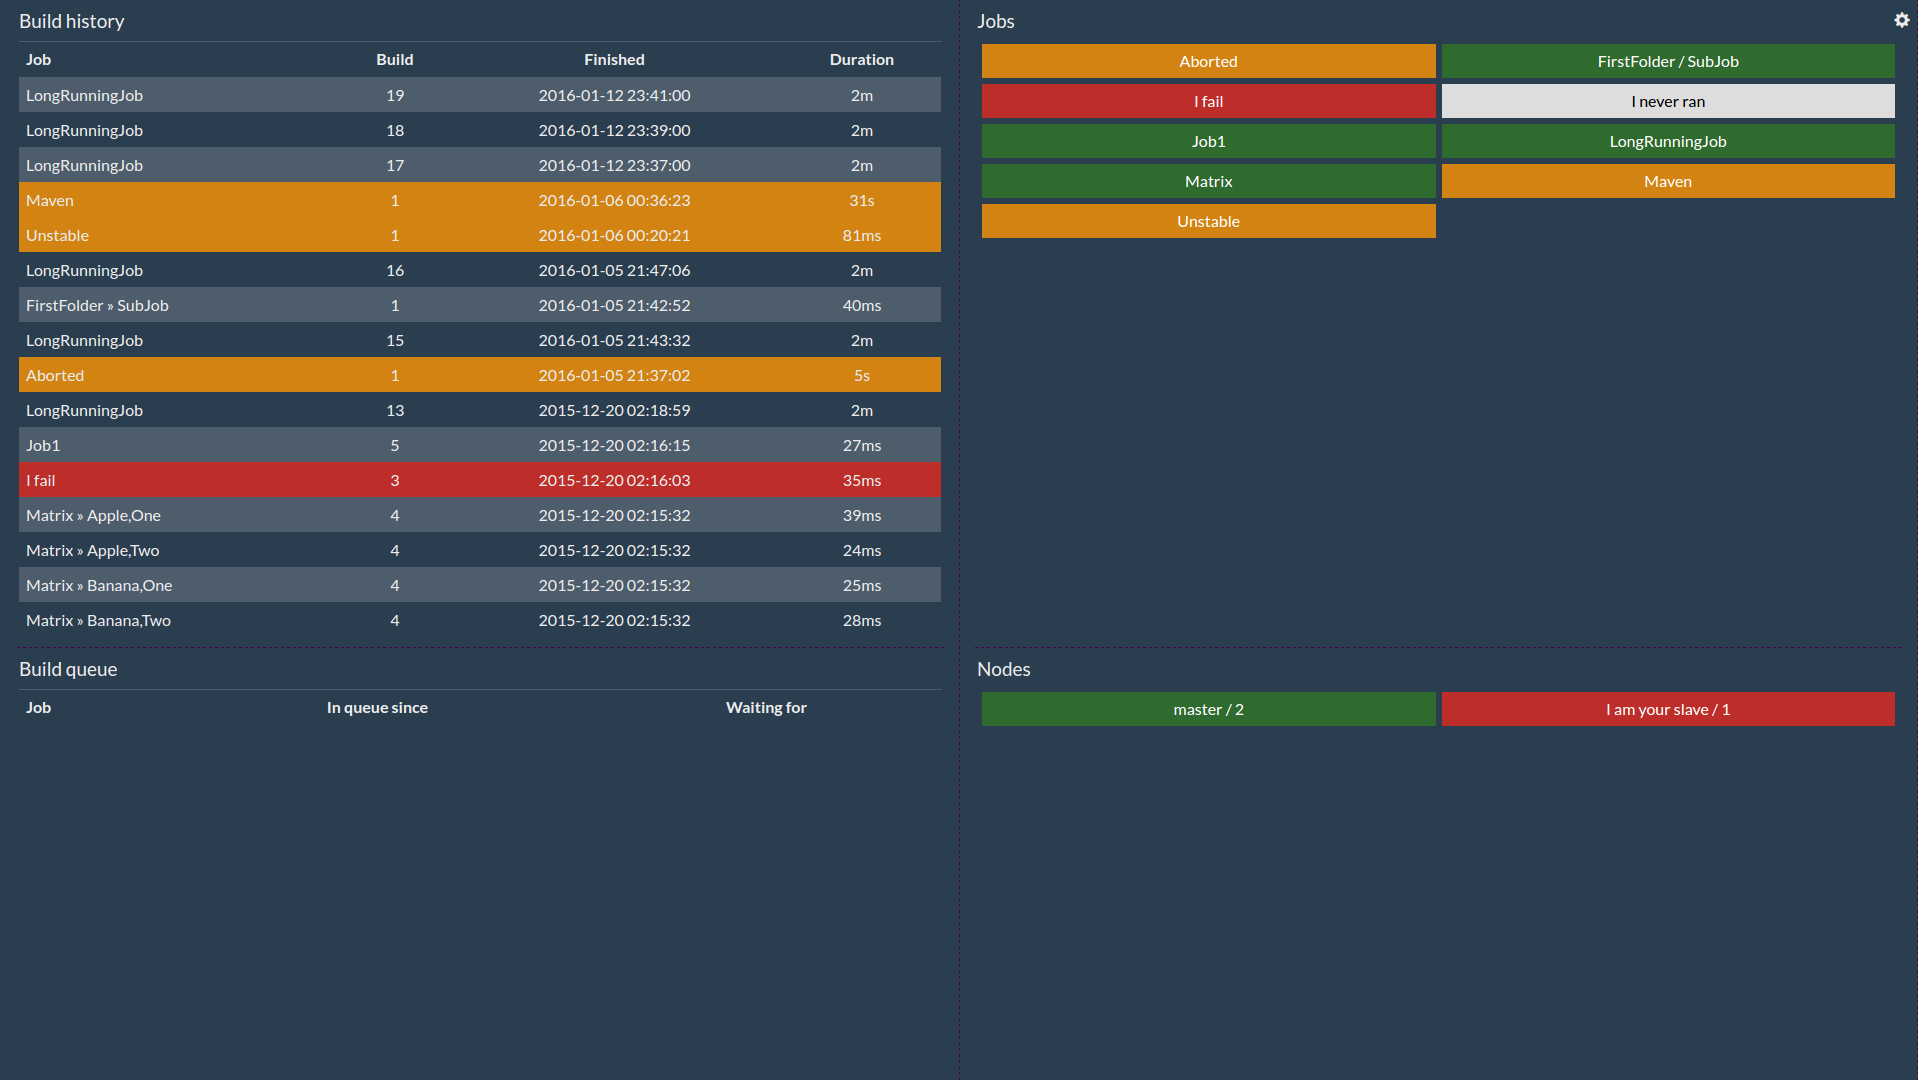
\includegraphics[width=1\textwidth]{missioncontrol}}
      \caption{Mission Control Plugin UI}
      \label{fig:missionControl}
  \end{figure}

\subsubsection{Metadata Plugin}\label{metadata_plugin}

Considering that one of the requirements is filtering the data displayed with the information of each test configuration, as said in section ~\ref{sec:res_system}, and since Jenkins has the possibility to store information on each of its CI items in XML format, exemplified in the figure~\ref{fig:buildXML}, then it could be stored some type of metadata as well.

To facilitate this, we used the extension point that Metadata Plugin~\cite{jkns:metadata} provides, in conjunction with the Jenkins API, to apply relevant filters on each job for an easier parsing of these configurations information.

  \begin{figure}[H]
  \centering
      \makebox[\textwidth][c]{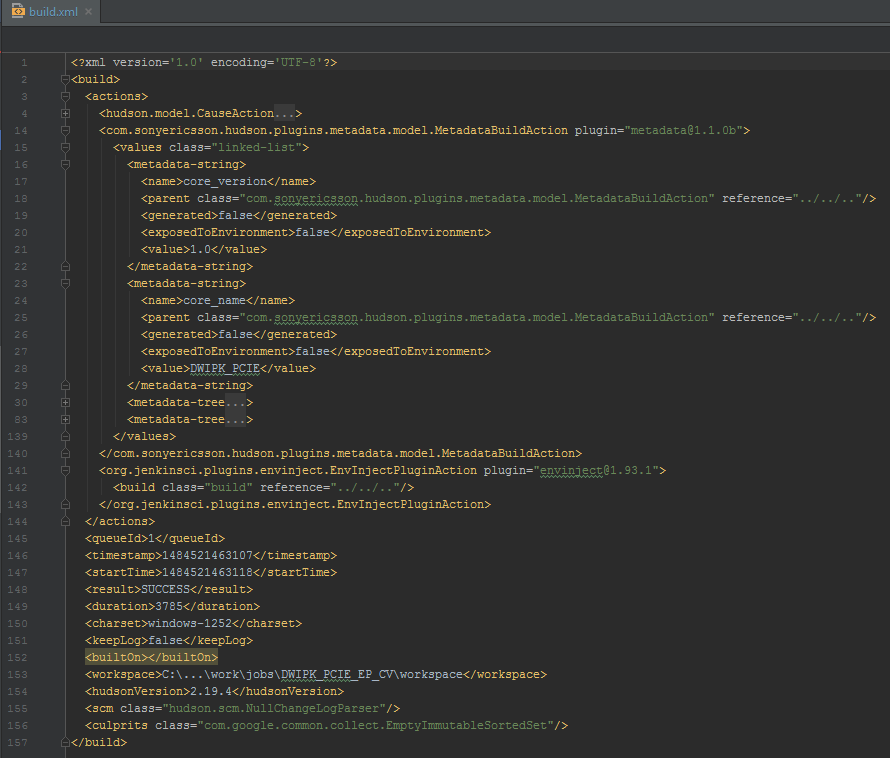
\includegraphics[width=1\textwidth]{buildXML}}
      \caption{XML file containing a Builds' information}
      \label{fig:buildXML}
  \end{figure}
  
This Metadata can be applied to Jobs simply through the customization menu, as seen in the figure~\ref{fig:metadataCustom}, which will apply it to every future Build after this point. 

  \begin{figure}[H]
  \centering
      \makebox[\textwidth][c]{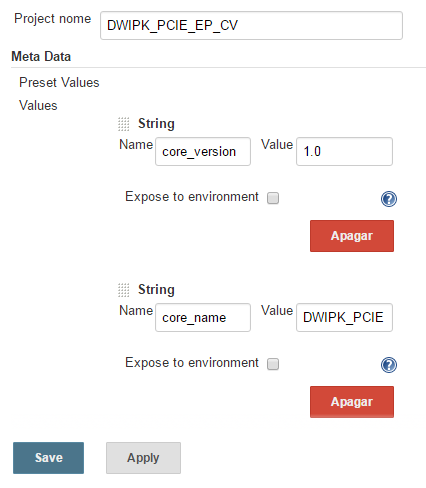
\includegraphics[width=0.5\textwidth]{metadataCustom}}
      \caption{Metadata option inside a Job customization panel}
      \label{fig:metadataCustom}
  \end{figure}

Or alternatively, automate the process simply by calling a post-build CLI command that is provided from the same plugin, using the format demonstrated in the figure~\ref{fig:updateMetadata}.

  \begin{figure}[H]
  \centering
      \makebox[\textwidth][c]{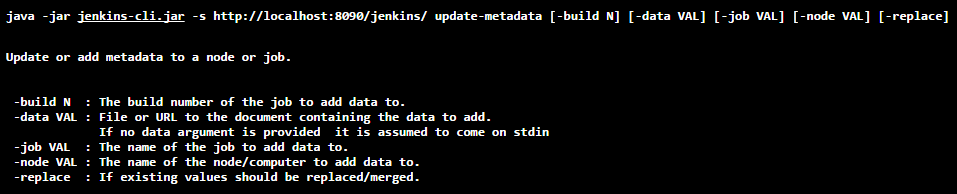
\includegraphics[width=1\textwidth]{updateMetadata}}
      \caption{CLI command update-metadata}
      \label{fig:updateMetadata}
  \end{figure}

\subsection{Server Side Implementation Design}\label{sc:implementationDesign}

Understanding how the back end in Java interacts with Jenkins and how projects were organized in Views, as explained in section \ref{sc:projOrg}, we defined a \textit{Top-down} strategy to obtain and parse the information of our items of interest.
This means we had to process View by View as individual projects to relate their child items in our Dashboard as seen in the figure~\ref{fig:dashboardDiagram}.

  \begin{figure}[H]
  \centering
      \makebox[\textwidth][c]{\includegraphics[width=1\textwidth]{dashboardDiagram}}
      \caption{\textit{Top-down} approach diagram}
      \label{fig:dashboardDiagram}
  \end{figure}
  
It was took in consideration the association between Views and Jobs inside Jenkins, namely that one Job is not associated to any View. Therefore each Job could be displayed multiple times, being represented by the same object.

We also needed a way to store information about the filters that can be applied, so we decided to implement a new Tag child in each Build. 

Based on this, our final plugin consists in this five different classes, depicted in the figure~\ref{fig:dash_uml}, that work together in parsing the information to display:

\begin{itemize}
\item \textbf{FilteredDashboardView - } The main class of the Dashboard. It collects all the Data from the Views selected and parses them into our other custom classes. After this collection, it exports the information to Jenkins API, which will be used to render and display in the front-end.

This class refreshes all the information when a new request is made by the front-end, which happens in a predefined time with an auto-refresh to capture new changes in the Jenkins instance, as schemed in the diagram \ref{fig:pluginInteraction}. 

We also ensure concurrency of the Views between all the life cycle of the class with a simple \code{CopyOnWriteArrayList<View> views = new CopyOnWriteArrayList<View>()} on its instantiation, which safeguards any View modification or deletion in the server. 

To ensure our approach scheme is followed, and prevent unnecessary duplicates of Jobs, these mapped in a variable \code{Map<String, JobData> jobsMap}, with their name serving as identifier, as well each Project mapped with its respective Jobs as \code{Map<String, ArrayList<String>> jobsInProjectMap}.

\item \textbf{Project - } Custom class representing a View. Contains a list of all Jobs inside the View as \code{ArrayList<JobData> projectJobs}. It is defined by its name \code{projectNane} and overall project status \code{projectStatus}. This status is calculated after all jobs are parsed and is set as the worst case scenario between them (i.e. if one Job fails, the whole project is set as \code{Fail}).

\item \textbf{JobData - } Custom class representing a Job. Contains a list of all Builds made by its represented Job as \code{ArrayList<Build> builds}. 

It has a subclass \textbf{JobVar} that keeps information of its variables, such as its URL, name and status. This concept was chosen for an easier access in the front-end, where we simply iterate through all these variables for display.

\item \textbf{Build -} Custom class representing a Build. Contains a list of Tags as  \code{ArrayList<Tag> tags} associated to this Build.

\item \textbf{Tag - } Class that represents a Metadata, from the plugin described in section ~\ref{metadata_plugin}, \code{label} and \code{value} contained in a Build, that will be used to apply filters in the Dashboard. Each \textbf{Tag} is the depiction of the configuration parameters utilized during the test process in section~\ref{sc:workflow}.
\end{itemize}

      \begin{figure}[H]
  \centering
      \makebox[\textwidth][c]{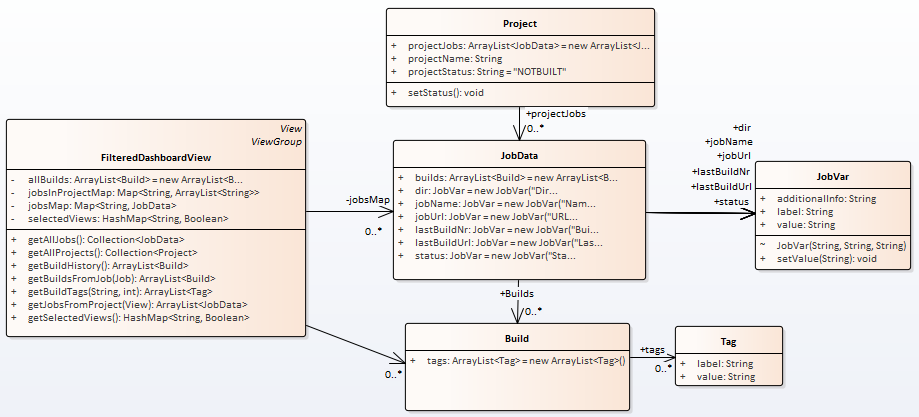
\includegraphics[width=1\textwidth]{dashboard_uml}}
      \caption{Filtered Dashboard View classes diagram}
      \label{fig:dash_uml}
  \end{figure}

      \begin{figure}[H]
  \centering
      \makebox[\textwidth][c]{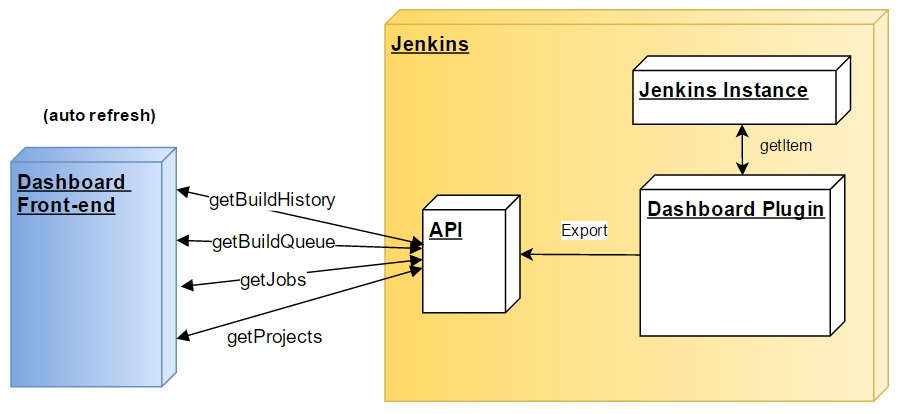
\includegraphics[width=1\textwidth]{frontBackConnection}}
      \caption{Interaction Diagram}
      \label{fig:pluginInteraction}
  \end{figure}

To eliminate some clustering of information, in the front-end we display only the last \textit{N} builds of each job. This number can be increased in the customization panel from figure \ref{fig:customize}, however it will also increase its processing time proportionally.

Finally, the addition of Tags to filter the information is the key feature of our Dashboard. This concept helps to maintain track of each configuration as requested in section \ref{sc:requirements}, with the minimum requisite of adding, or modifying, these labels to Jobs in the building process.

This design permits a totally scalable structure, since it has no limitations on the number of Views associated to the Dashboard, nor its Jobs and Builds. It can also be extendable to put more information in each of its custom classes for additional metrics and indicators in the future if desired. All this information only depends on the Jenkins API and what it supports.

\subsection{Front-End Implementation Design}\label{sc:frontend}

After the development of the server side, it was needed some brainstorming on how to organize the information structured and display it in the browser. 

For this, in the front-end display of the Dashboard, we based on the same scripts of the Mission Control Plugin, described in section~\ref{mission_plugin}, along with several common Web Application libraries and frameworks such as Javascript, jQuery and Bootstrap, all processed in Apache Jelly~\cite{jelly}, a Java and XML based scripting and processing engine that allows Jenkins its UI to be extended by plugins.

Since the data exported to the API is already well structured, the presentation process was completed with ease, only requiring a way to exhibit the view of a project with an intuitive display. 

To accomplish the aforementioned, was decided to display every Job inside the project as a column in a table, using the library referenced in section~\ref{sc:datatables}, being each row cell its Builds organized in a descending chronological order. Each cell has its Tags associated for a quick reference of the configurations utilized in the respective Build.



\subsubsection{Auxliary Library: DataTables - jQuery}\label{sc:datatables}

DataTables~\cite{dataTables} is a plugin for the jQuery Javascript library. 
It is a highly flexible tool that helped to create and add advanced interaction controls to any HTML table.

Is one of the key components of the front-end that made possible and simple the creation of a display table within the Dashboard, as well the search interaction with the added Tag filters.

\subsubsection{User Interface}\label{sc:ui}

Once the Dashboard is selected, it displays every View selected previously, as seen in the figure \ref{fig:createView}, and the overall status of those projects. It also shows all the Jobs inside those Views, and a Build history resulted from these, organized chronologically from the most recent. It is to note that every one of this items is linked directly to its object inside the Jenkins tool, eliminating the need of searching for them in the system.
  
In the figure~\ref{fig:mainDashb} its is shown the Synopsys IPK R\&D team's Dashboard, which are associated both HDMI and PCIe projects.
  
\begin{figure}[H]
  \centering
      \makebox[\textwidth][c]{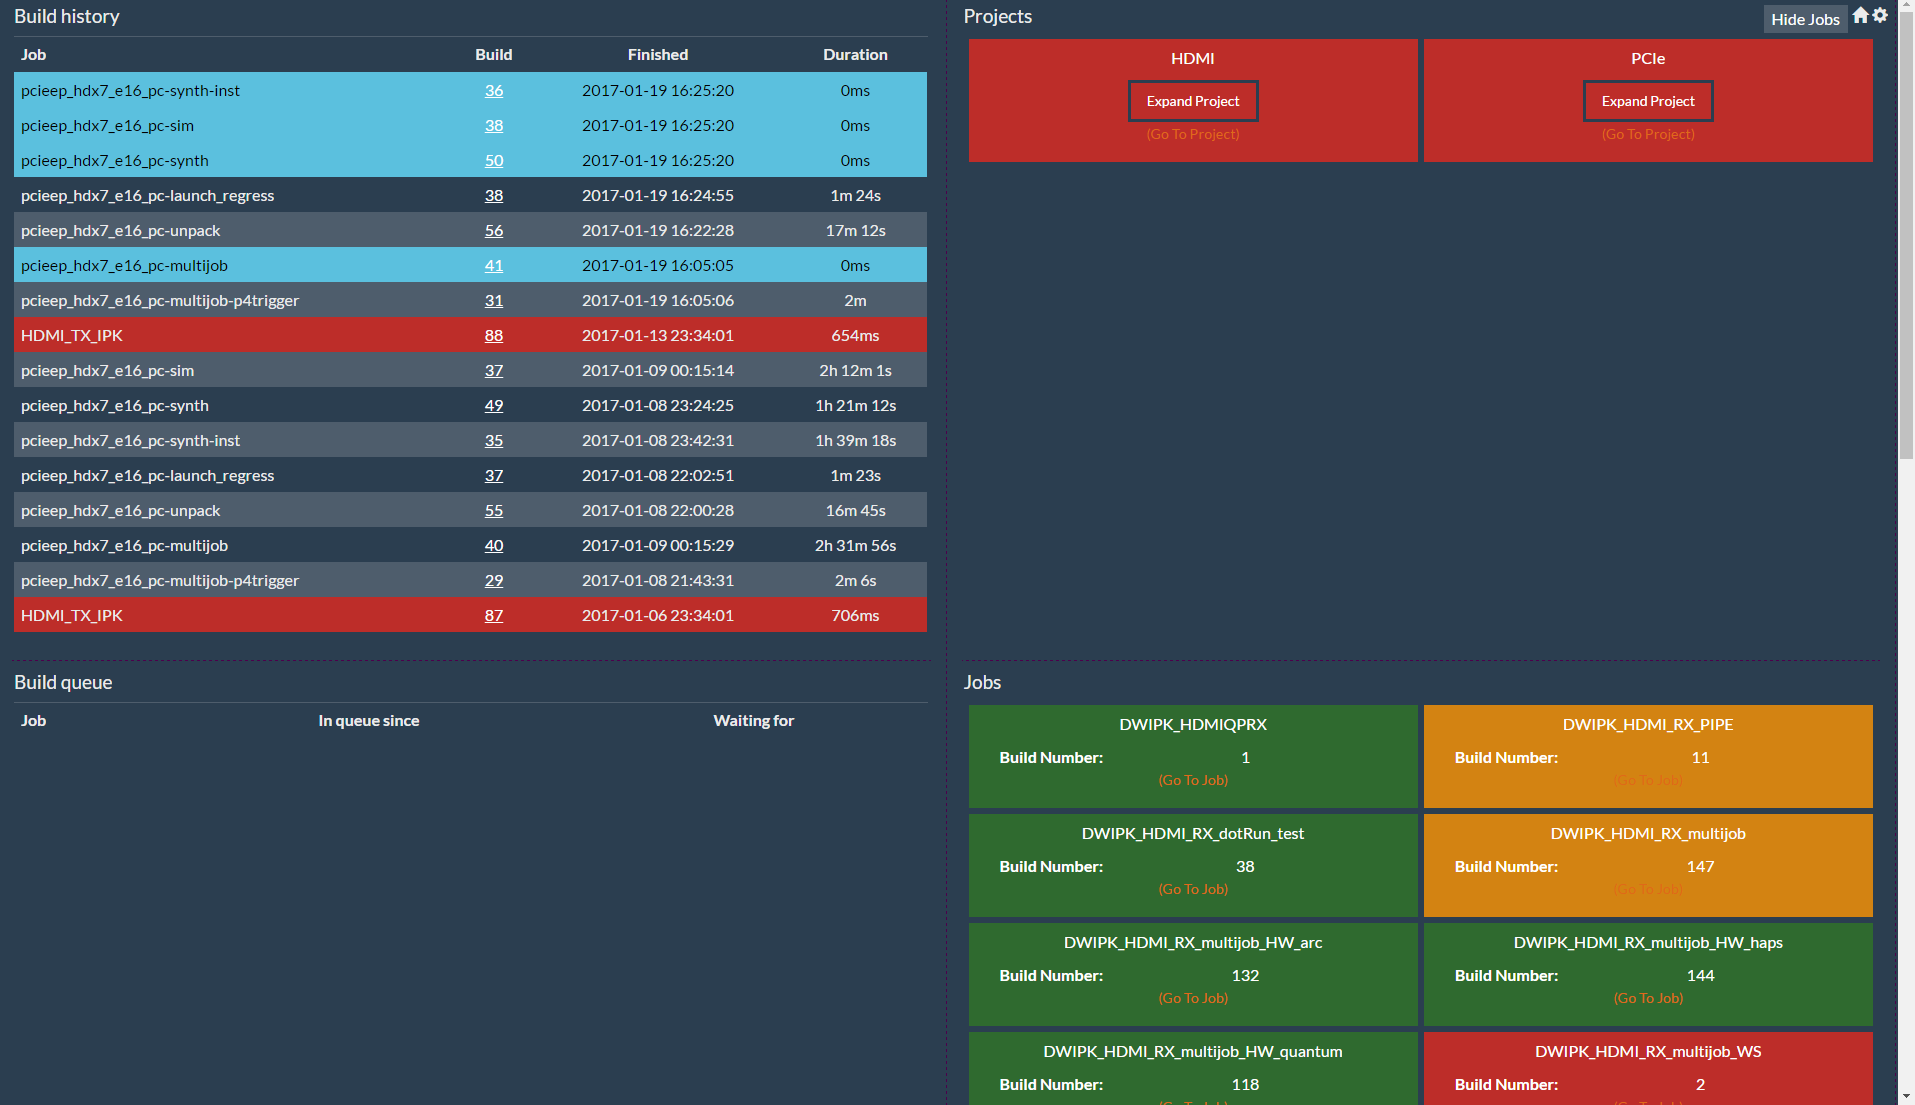
\includegraphics[width=1\textwidth]{maindashboard}}
      \caption{Dashboard Landing page}
      \label{fig:mainDashb}
  \end{figure}
  
It displays a "straight to the point" facet, that helps to identify exactly which Job or Build is not corresponding to the expected results.
 
  
Inside of each sub-view, the user can see information about Jobs, Builds and overall Project status, as well as the different filters defined by the Metadata inputs, referring to the different test configurations, displayed in the figure~\ref{dashboardTable1}. 
  
\begin{figure}[H]
  \centering
      \makebox[\textwidth][c]{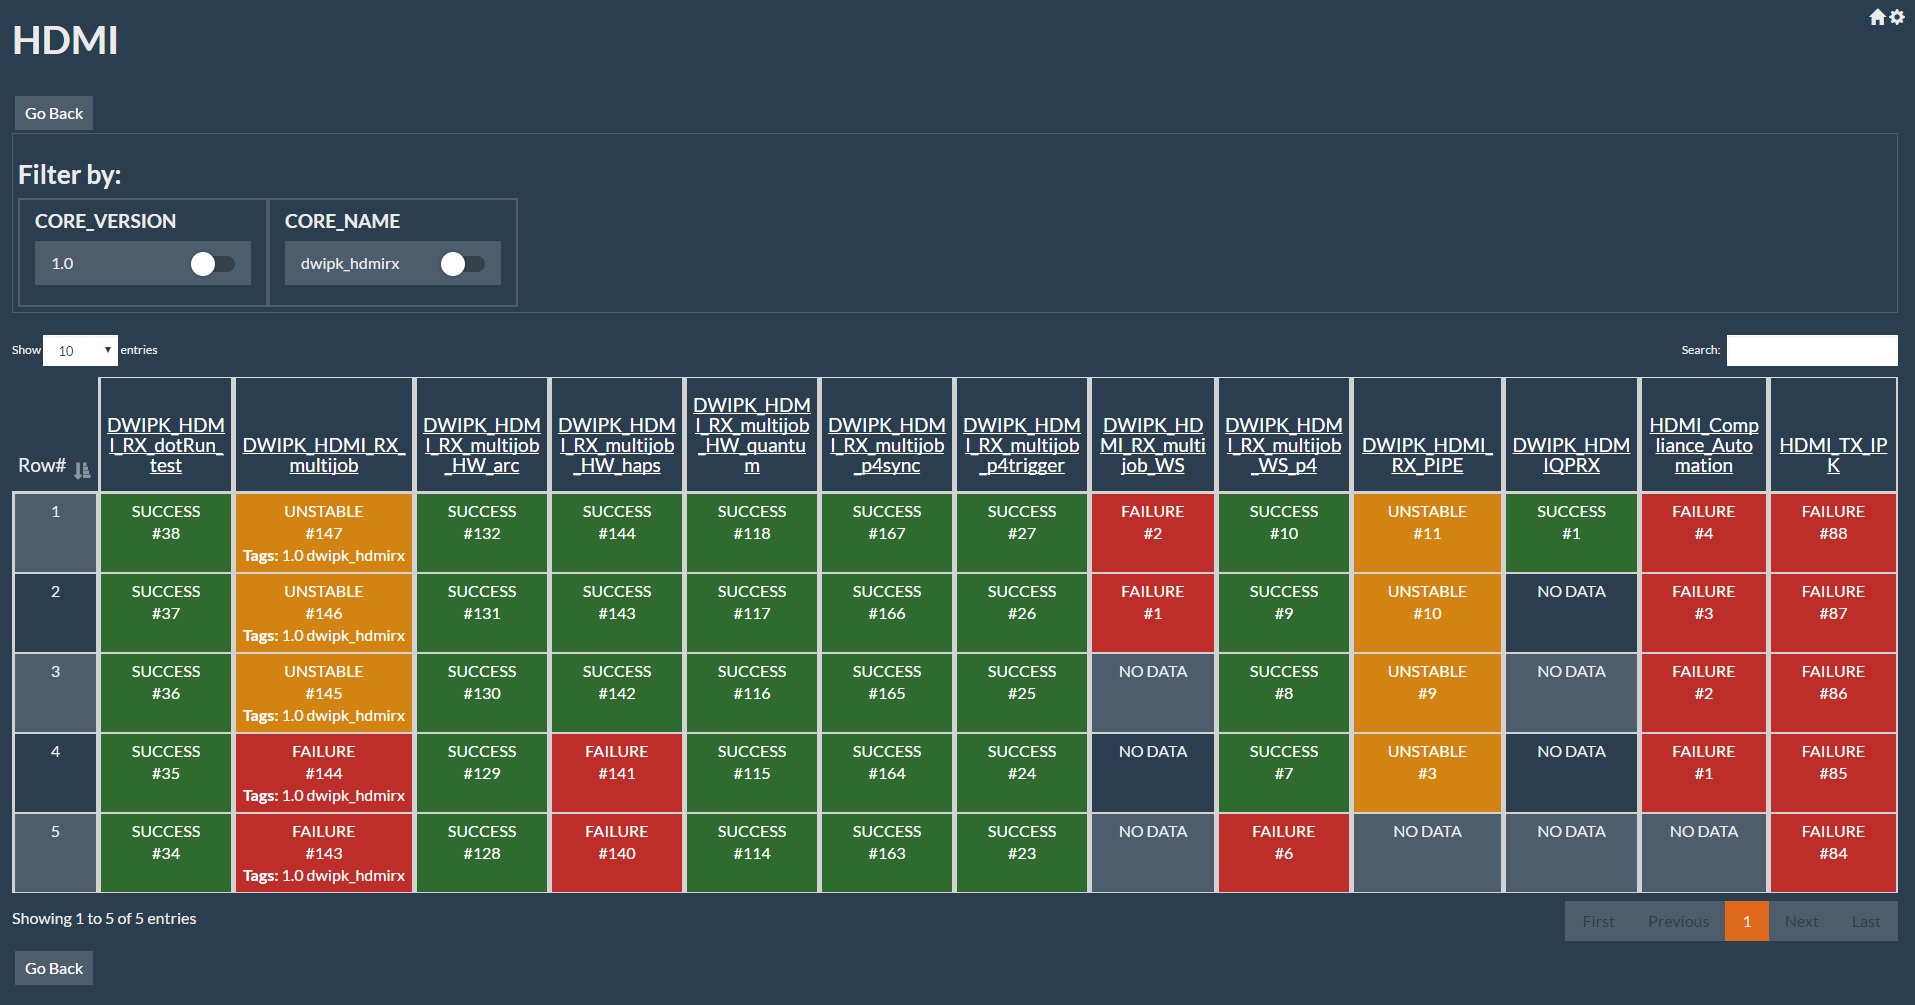
\includegraphics[width=1\textwidth]{dashboardtable1}}
      \caption{Overall view of a Project}
      \label{dashboardTable1}
  \end{figure}
  
For a quick filtering through the Tags, the user simply needs to select them in the respective section (Fig. \ref{dashboardTable2}). This search is made following a regular expression using the \code{AND} operator through all the selected Tags, displaying only the Builds that follow it. With this, we attain the desired streamlined perspective to troubleshoot and validate the configurations.
  
\begin{figure}[H]
  \centering
      \makebox[\textwidth][c]{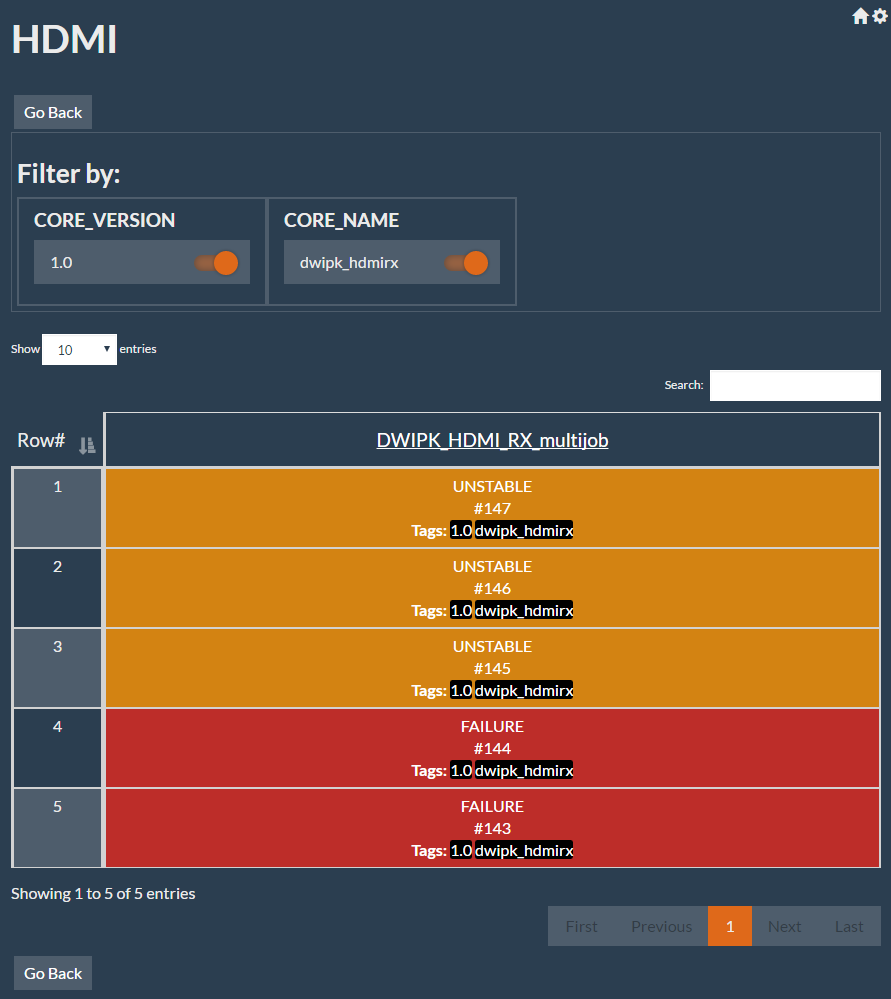
\includegraphics[width=0.6\textwidth]{dashboardtable2}}
      \caption{Overall view of the same Project (Fig.~\ref{dashboardTable1}) with filters applied}
      \label{dashboardTable2}
  \end{figure}

\section{Metadata and Pipeline Workaround}\label{workaraound}

One issue that was discovered while developing our plugin, was the incompatibility between the Metadata Plugin, from section \ref{metadata_plugin}, and the Pipeline Jobs~\cite{jnks:pipeline}. This occurs because the Metadata Plugin only supports Abstract Jobs, while Workflow Jobs (created in Pipeline) are not inherited from this class, since it was created in a pre-Workflow era.

To workaround this problem, it was created a function, exemplified in the snippet~\ref{groovy:setMetadata}, that can be patched in Pipeline Jobs groovy scripts and still maintain their complete functionality while being used in our Dashboard.

For this, one has to allow Pipeline builds to be Parameterized, as seen in figure \ref{fig:param}, and add String Parameters with the following structure: \(\textbf{metadata:}name\), where \(name\) can be any string the user wishes to reference the name of the metadata. This is valid because the inclusion of both Metadata and Parameters in Builds, are extended from the \code{Action} extension point of Jenkins.
Afterwards, only this function is needed in the Groovy script.

\begin{figure}[H]
  \centering
      \makebox[\textwidth][c]{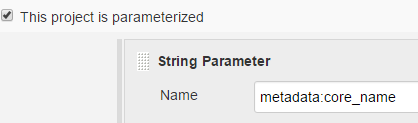
\includegraphics[width=0.6\textwidth]{parametrized}}
      \caption{Parameterized project selection}
      \label{fig:param}
  \end{figure}

\begin{lstlisting}[language=Java, label=groovy:setMetadata, caption=Groovy Script Workaround]
import hudson.model.*

@NonCPS
def setMetadata(map){
    def npl = new ArrayList<ParametersAction>();
    for(e in map){
        npl.add(new StringParameterValue(e.key.toString(), e.value.toString()));
    }
    def newPa = null
    def oldPa = currentBuild.build().getAction(ParametersAction.class)
    if (oldPa != null) {
        currentBuild.build().actions.remove(oldPa)
        newPa = oldPa.createUpdated(npl)
    } else {
        newPa = new ParametersAction(npl)
    }
    currentBuild.build().actions.add(newPa);
}
def map = [:]

//Example to populate the map:
map['metadata:core_name'] = 'DWIPK_HDMI_RX';
map['metadata:core_version'] = '1.0';
setMetadata(map);
\end{lstlisting}

This information will be parsed inside our dashboard with a condition statement, displayed in our snippet~\ref{java:pipelineIf} function, that creates exactly the same output for Pipelines as if other Job was being processed.

\begin{lstlisting}[language=Java, label=java:pipelineIf, caption=Java Condition Statement Workaround]
    public ArrayList<Tag> getBuildTags(String jobName, int buildNr) {
        ArrayList<Tag> tags = new ArrayList<Tag>();
        Job job = Jenkins.getInstance().getItemByFullName(jobName, Job.class);
        Run build = job.getBuildByNumber(buildNr);
        
        if (job.getClass().getName().equals("org.jenkinsci.plugins.workflow.job.WorkflowJob")) {
            ParametersAction parameterActions = build.getAction(ParametersAction.class);
            if (parameterActions != null) {
                for (ParameterValue parameter : parameterActions.getAllParameters()) {
                    if (parameter.getClass().equals(StringParameterValue.class)) {
                        if (StringUtils.substring(parameter.getName(), 0, "metadata:".length()).equals("metadata:") &&
                                !parameter.getValue().equals("")) {
                            String name = parameter.getName().replace("metadata:", "");
                            tags.add(new Tag(name.toUpperCase(), parameter.getValue().toString().toLowerCase()));
                        }
                    }
                }
            }
        }...        
      }      
\end{lstlisting}

\section{Conclusion}\label{sc:conclusion}

In this chapter the Dashboard solution was fully detailed along with the fixes one must do to make it fully functional with Pipelines. It is divided in simple classes that can be used as base for future extensions to the main View.

We can safely disclose that every obstacle in the previous Spreadsheet solution, detailed in section~\ref{sec:spreadsheet}, was surpassed:

\begin{itemize}
\item \textbf{Traceability - } The Dashboard is automatically updated when a new test is made.
\item \textbf{Susceptible to Human Error - } All the information comes from inside Jenkins, so there is no human interference in the process of displaying the information.
\item \textbf{Availability - } The only requirement is being a user inside the Jenkins tool and having permission to see the View.
\item \textbf{Difficulty to troubleshoot - } Every item on the Dashboard is linked directly to the original inside Jenkins, making the process a "one click" distance.
\end{itemize}

The plugin is made abstract enough so it can be used not only by our main target environment, but to help other software development teams equally.